\documentclass[12pt,a4paper]{article}
\usepackage[utf8]{inputenc} %polskie znaki
\usepackage[T1]{fontenc}	%polskie znaki
\usepackage{amsmath}		%matematyczne znaczki :3
\usepackage{enumerate}		%Dodatkowe opcje do funkcji enumerate
\usepackage{geometry} 		%Ustawianie marginesow
\usepackage{graphicx}		%Grafika
\usepackage{wrapfig}		%Grafika obok textu
\usepackage{float}			%Allows H in fugire
\pagestyle{empty} 			%usuwa nr strony

\newgeometry{tmargin=2cm, bmargin=2cm, lmargin=2cm, rmargin=2cm} 

\begin{document}
	\begin{center}
		\LARGE Planimetria - sprawdzian
	\end{center}
	\vspace{1.5cm}
	\begin{flushright}
		\textbf{2 TERMIN}
	\end{flushright}
	\begin{tabular}{p{13cm} r}
		Imię i nazwisko: ............................................................................
		&[....../30pkt]\\ 
		\vspace{0.5cm}
	\end{tabular}
	\begin{enumerate}[1.]
		\item  \begin{tabular}{p{13cm} r}	%Zad1
			Oblicz "x", "y" i "z": &[4pkt]\\ 
		\end{tabular}
		\begin{figure}[h]
			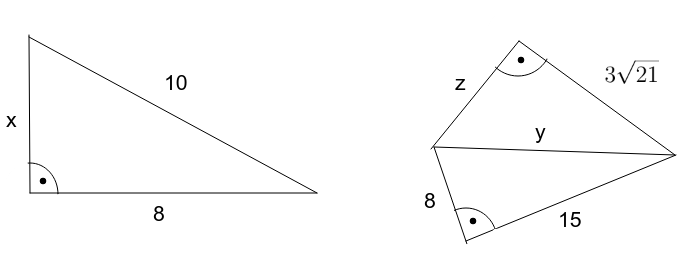
\includegraphics[scale=0.8]{tp1}
		\end{figure}
		
		\item  \begin{tabular}{p{13cm} r}	%Zad2
			Oblicz kąty $\alpha$, $\beta$, $\gamma$, $\delta$: &[4pkt]\\ 
		\end{tabular}
		\begin{figure}[h]
			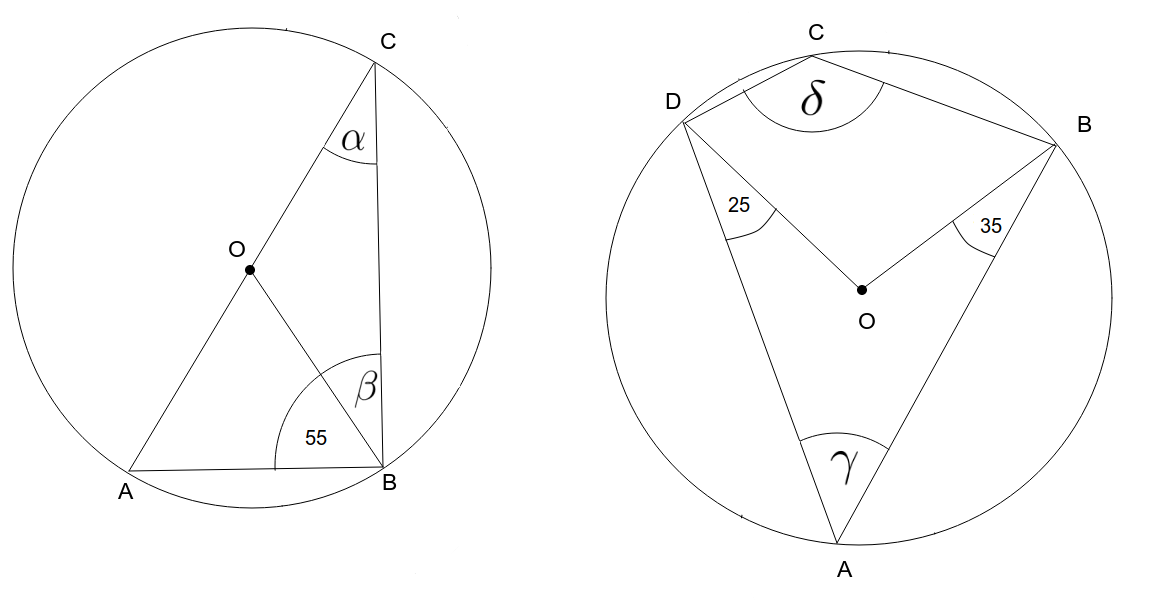
\includegraphics[scale=0.4]{p2}
		\end{figure}
		
		\newpage
		
		\item  \begin{tabular}{p{13cm} r}	%Zad3
			Oblicz promień okręgu opisanego na trójkącie prostokątnym o przyprostokątnych długości 10cm i 24cm.&[4pkt]\\ 
		\end{tabular}
		
		\item  \begin{tabular}{p{13cm} r}	%Zad4
			Oblicz obwód trapezu równoramiennego: &[6pkt]\\ 
		\end{tabular}
		\begin{figure}[h]
			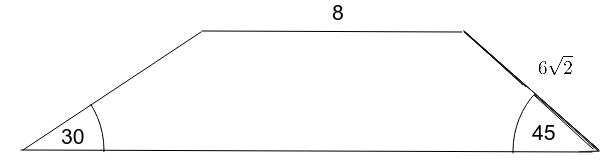
\includegraphics[scale=0.8]{tp3}
		\end{figure}
		
		\item  \begin{tabular}{p{13cm} r}
			Jeden z boków prostokąta jest pięć razy dłuży od drugiego. Wiedząc, że przekątna tego prostokąta jest równa 26, oblicz jego pole. &[4pkt]\\
		\end{tabular}
		
		\item  \begin{tabular}{p{13cm} r}
			Jedna z dwusiecznych trójkąta równobocznego ma długość 18. Wyznacz bok tego trójkąta. &[4pkt]\\ 
		\end{tabular}
		
		\item  \begin{tabular}{p{13cm} r}
			W okręgu o promieniu $4\sqrt{2}$ wpisano kwadrat. Oblicz promień koła wpisanego w kwadrat. &[4pkt]\\ 
		\end{tabular}
	\end{enumerate}
	
\end{document}
